\documentclass[
    a4paper,
    12pt,
    addpoints,
    % answers,
    noanswers,
    hidelinks,
]
{exam}

%%% Packages and macros

\usepackage{1-preamble}

%%% Page layout

%%% Width

\extrawidth{.5in}

%%% Header and footer (cover pages)

\coverextraheadheight{2in}

\coverheader{}{\bfseries\large Test Supervision Instructions}{}
\coverfooter{}{\thepage}{}

%%% Header and footer (main)

\headrule
\lhead[\bfseries Name:\\Supervisor:]{\bfseries OAC \subject}
\chead{}
\rhead[\bfseries \papername\\\paperrules]{\iflastpage{\bfseries Extra Space \& Mathematical Formul\ae}{\bfseries \papernameshort}}
\lfoot{\scriptsize $\mathfrak{P}\mathfrak{L}\mathfrak{G}$\\\RNum{\year}}
\cfoot{\iflastpage{Page \thepage\ of \pageref{LastPage}\\End of paper}{Page \thepage\ of \pageref{LastPage}}}
\rfoot{\iflastpage{}{Score: \makebox[.375in]{\hrulefill} /\pointsonpage{\thepage}}}

%%% Points

\boxedpoints
\pointsinrightmargin
     
%%% Solutions

\SolutionEmphasis{
	\small
}       
\shadedsolutions
\definecolor{SolutionColor}{rgb}{0.8,0.9,1}


%%% Subject, paper and conditions

\newcommand{\subject}{Stage 2 Specialist Mathematics}
\newcommand{\papername}{SAT: 3D Vectors (Practise)}
\newcommand{\papernameshort}{3D Vectors (Practise)}
\newcommand{\timelimit}{$\infty$~Minutes}
\newcommand{\conditions}{Notes, Calculator}
\newcommand{\paperrules}{\timelimit, \conditions}

\begin{document}

% \begin{coverpages}

\noindent \today

\vspace{.375in}

\noindent Dear test supervisor:

\vspace{.125in}

\noindent Thanks for supporting student learning at OAC! Please remind students to use a blue or black pen throughout and to draw graphs accurately in pencil. Students should show all their working.

\vspace{.125in}

\noindent Make sure that you both \textbf{write your names} in the space provided on Page~1, to indicate that these exam conditions were satisfied:
\begin{itemize}
    \item Time limit: \textbf{\MakeLowercase \timelimit}.
    \item Restrictions: \textbf{\MakeLowercase \conditions\ allowed}.
	\item Students shouldn't use the internet.
	\item Students shouldn't discuss their work with anyone.
\end{itemize}

\vspace{.125in}

\noindent This page can be removed before you distribute the test to students. Scan and email the completed test back to me by the due date. If the extra space wasn't used, it needn't be returned.

\vspace{.125in}

\noindent Sincerely,

\vspace{.75in}

\noindent Peter Gent \\
Open Access College

\end{coverpages}



\begin{questions}

\question % 2010 Exam, Q8.
Consider the equilateral triangle $ABC$ shown in Figure~\ref{fig:equilateral-triangle-with-vectors}. Let $\vv{AC} = \vec{c}$ and let $\vv{AB} = \vec{b}$.

\begin{figure}[h]
	\centering
	\begin{tikzpicture}[scale=.75]
	\ifprintanswers
	\tkzDefPoints{0/0/A, 4/0/B}
	\tkzDefTriangle[equilateral](A,B)
	\tkzGetPoint{C}
	\tkzDrawPolygon[semithick](A,B,C)
	\tkzLabelPoints[left](A)
	\tkzLabelPoints[right](B)
	\tkzLabelPoints[above](C)
	\tkzDefPointWith[colinear=at B,K=2](C,A)
	\tkzGetPoint{D}
	\tkzLabelPoints[red](D)
	\tkzDrawSegment[vector,red](A,C)
	\tkzDrawSegment[vector,red](A,B)
	\tkzDrawSegment[vector,red](B,D)
	\tkzDrawSegment[vector,gray](A,D)
	\tkzLabelSegment[left,red](A,C){$\vec{c}$}
	\tkzLabelSegment[below,red](A,B){$\vec{b}$}
	\tkzLabelSegment[red](B,D){$-2\vec{c}$}
	\tkzLabelSegment[gray,left](A,D){$\vec{b} - 2\vec{c}$}
	\tkzMarkRightAngle(D,A,B)
	\else
	\tkzDefPoints{0/0/A, 4/0/B}
	\tkzDefTriangle[equilateral](A,B)
	\tkzGetPoint{C}
	\tkzDrawPolygon[semithick](A,B,C)
	\tkzLabelPoints[left](A)
	\tkzLabelPoints[right](B)
	\tkzLabelPoints[above](C)
	\tkzDefPointWith[colinear=at B,K=2](C,A)
	\tkzGetPoint{D}
	\tkzDrawSegment[vector,red,opacity=0](B,D)
	\fi
	\end{tikzpicture}
	\caption{An equilateral triangle.}
	\label{fig:equilateral-triangle-with-vectors}
\end{figure}

\begin{parts}

\part[1]
Draw the vector $\vv{BD} = -2\vec{c}$ on Figure~\ref{fig:equilateral-triangle-with-vectors}.

\part[3]
Prove that $\vec{b} \cdot (\vec{b} - 2\vec{c}) = 0$.

\begin{EnvFullwidth}
\begin{solutionorgrid}[1.5in]
\begin{proof}
We have
\begin{align*}
    \vec{b} \cdot (\vec{b} - 2\vec{c}) &= \vec{b} \cdot \vec{b} - 2\vec{b} \cdot \vec{c} \\
    &= \abs{\vec{b}}^2 - \cancel{2}\abs{\vec{b}}\abs{\vec{c}}\cancel{\cos(\ang{60})} \\
    &= \abs{\vec{b}}^2 - \abs{\vec{b}}\abs{\vec{b}} && (\abs{\vec{c}} = \abs{\vec{b}}) \\
    &= 0.
\end{align*}
\end{proof}
\end{solutionorgrid}
\end{EnvFullwidth}

\part[2]
Illustrate the result from part (b).

\end{parts}

\threeast

\question % HL (Core) - Third Edition, RS 15C, Q14.
Let $t$ be a real number and let
\[
	\ell_1 : \frac{x - 3}{2} = y - 4 = \frac{z + 1}{-2}
	\qquad
	\ell_2 :
	\begin{cases}
		x(t) = -1 + 3t \\
		y(t) = 2 + 2t \\
		z(t) = 3 - t
	\end{cases}
\]
be two lines.

\begin{parts}

\part[1]
Find direction vectors for both lines.

\begin{EnvFullwidth}
\begin{solutionorgrid}[.75in]
Direction vectors are
\[
	\vec{d}_1 = \colvec{3}{2}{1}{-2}, \qquad \vec{d}_2 = \colvec{3}{3}{2}{-1}.
\]
\end{solutionorgrid}
\end{EnvFullwidth}

\part[1]
Hence, show that the two lines are not parallel.

\begin{EnvFullwidth}
\begin{solutionorgrid}[1.5in]
Let $k$ be a real number. Since
\[
    \vec{d}_1 \neq k \vec{d}_2
\]
the lines aren't parallel.
\end{solutionorgrid}
\end{EnvFullwidth}

\part[3]
Find the point of intersection $P$ of $\ell_1$ and $\ell_2$.

\begin{EnvFullwidth}
\begin{solutionorgrid}[2in]
For real numbers $s$ and $t$
\[
	\ell_1 :
	\begin{cases}
		x(s) = 3 + 2s \\
		y(s) = 4 + s \\
		z(s) = -1 - 2s
	\end{cases},
	\qquad
	\ell_2 :
	\begin{cases}
		x(t) = -1 + 3t \\
		y(t) = 2 + 2t \\
		z(t) = 3 - t.
	\end{cases}
\]
By solving for $s$, we get
\[
	s = \frac{-1 + 3t - 3}{2} = 2 + 2t - 4 = \frac{3 - t + 1}{-2}.
\]
This is true for $t = 0$. So the point is $P(-1, 2, 3)$.
\end{solutionorgrid}
\end{EnvFullwidth}

\end{parts}


\threeast

\question % 2005 Exam, Q5.
Figure~\ref{fig:proof-of-parallel-lines} shows triangle $OAB$ with vectors $\vv{OA} = \vec{a}$ and $\vv{OB} = \vec{b}$. Points $X$ and $Y$ lie on $OB$ and $AB$ such that $OX = 4XB$ and $AY = 4YB$.

\begin{figure}[h]
    \centering
    \begin{tikzpicture}
    \tkzDefPoints{0/0/O, 5/.8/A, 3/4/B}
    \tkzDefPointWith[colinear=at O,K=0.8](O,B)
    \tkzGetPoint{X}
    \tkzDefPointWith[colinear=at A,K=0.8](A,B)
    \tkzGetPoint{Y}
    \tkzDrawPolygon(O,A,B)
    \tkzDrawSegment(X,Y)
    \tkzLabelPoints[below left](O)
    \tkzLabelPoints(A)
    \tkzLabelPoints[above right](B)
    \tkzLabelPoints[left](X)
    \tkzLabelPoints[right](Y)
    \ifprintanswers
    \tkzDrawSegment[vector,red](O,A)
    \tkzDrawSegment[vector,red](O,B)
    \tkzLabelSegment[below,red](O,A){$\vec{a}$}
    \tkzLabelSegment[left,red](O,B){$\vec{b}$}
    \else
    \fi
    \end{tikzpicture}
    \caption{The area of these two triangles will be compared.}
    \label{fig:proof-of-parallel-lines}
\end{figure}

\begin{parts}

\part
Find in terms of $\vec{a}$ and $\vec{b}$ the vectors:

\begin{subparts}

\subpart[1]
$\vv{AB}$.

\begin{EnvFullwidth}
\begin{solutionorgrid}[1in]
We have
\[
    \vv{AB} = \vec{b} - \vec{a}.
\]
\end{solutionorgrid}
\end{EnvFullwidth}

\subpart[1]
$\vv{OX}$.

\begin{EnvFullwidth}
\begin{solutionorgrid}[1in]
We have
\[
    \vv{OX} = \frac{4}{5}\vec{b}.
\]
\end{solutionorgrid}
\end{EnvFullwidth}

\end{subparts}

\part[2]
Use a vector proof to show that $XY$ is parallel to $OA$.

\begin{EnvFullwidth}
\begin{solutionorgrid}[2in]
\begin{proof}
By part (a)
\begin{align*}
    \vv{XY} &= -\vv{OX} + \vv{OA} + \frac{4}{5}\vv{AB} \\
    &= -\frac{4}{5}\vec{b} + \vec{a} + \frac{4}{5}(\vec{b} - \vec{a}) \\
    &= \frac{1}{5}\vec{a},
\end{align*}
which is a scalar multiple of $\vec{a}$.
\end{proof}
\end{solutionorgrid}
\end{EnvFullwidth}

\part
If $\abs{\vec{a} \times \vec{b}} = 4$, find the area of:

\begin{subparts}

\subpart[1]
triangle $OAB$.

\begin{EnvFullwidth}
\begin{solutionorgrid}[1in]
The area of triangle $OAB$ is
\[
    \frac{1}{2}\abs{\vec{a} \times \vec{b}} = 2 \, \textrm{units}^2.
\]
\end{solutionorgrid}
\end{EnvFullwidth}

\subpart[2]
triangle $XYB$.

\begin{EnvFullwidth}
\begin{solutionorgrid}[1.5in]
The area of a triangle is $\frac{1}{2}ab\sin(\gamma)$. Triangles $OAB$ and $XYB$ are similar so
\[
    \angle{BOA} = \gamma = \angle{BXY}.
\]
The side lengths are $\frac{1}{5}$ of what they were before, so triangle $XYB$ has area
\[
    \frac{1}{5} \times \frac{1}{5} \times 2 = \frac{2}{25} \, \textrm{units}^2.
\]
\end{solutionorgrid}
\end{EnvFullwidth}

\end{subparts}

\end{parts}


\triast

\uplevel{
\begin{proposition}[Dot product of vector sum with itself]
\label{prop:dot-product-of-vector-sum-with-itself}
Let $\vec{u}$ and $\vec{v}$ be vectors. Then
\[
    (\vec{u} + \vec{v}) \cdot (\vec{u} + \vec{v}) = \abs{\vec{u} + \vec{v}}^2.
\]
\end{proposition}
}

\question % 2013 Exam, Q6.
Let $\vec{a} = \colvec{3}{1}{2}{-4}$ and $\vec{b} = \colvec{3}{5}{-3}{-2}$ be vectors.

\begin{parts}

\part

\begin{subparts}

\subpart[1]
Find $\abs{\vec{a}}$.

\begin{EnvFullwidth}
\begin{solutionorgrid}[1in]
We have
\[
    \abs{\vec{a}} = \sqrt{1^2 + 2^2 + (-4)^2} = \sqrt{21}.
\]
\end{solutionorgrid}
\end{EnvFullwidth}

\subpart[1]
Find $\vec{a} \cdot \vec{b}$.

\begin{EnvFullwidth}
\begin{solutionorgrid}[1in]
We have
\[
    \vec{a} \cdot \vec{b} = 1 \times 5 + 2 \times (-3) + (-4) \times (-2) = 7.
\]
\end{solutionorgrid}
\end{EnvFullwidth}

\subpart[2]
Verify that $\abs{\vec{a} + \vec{b}}^2 = \abs{\vec{a}}^2 + \abs{\vec{b}}^2 + 2\vec{a} \cdot \vec{b}$.

\begin{EnvFullwidth}
\begin{solutionorgrid}[2.5in]
The LHS is
\[
    (\sqrt{6^2 + (-1)^2 + (-6)^2})^2 = 73,
\]
and, by parts (a)(i) and (ii), the RHS is
\[
    (\sqrt{21})^2 + (\sqrt{38})^2 + 2 \times 7 = 73.
\]
\end{solutionorgrid}
\end{EnvFullwidth}

\end{subparts}

\part[2]
Use Proposition~\ref{prop:dot-product-of-vector-sum-with-itself} to show that $\abs{\vec{u} + \vec{v}}^2 = \abs{\vec{u}}^2 + \abs{\vec{v}}^2 + 2\vec{u} \cdot \vec{v}$ for \emph{all} vectors $\vec{u}$ and $\vec{v}$.

\begin{EnvFullwidth}
\begin{solutionorgrid}[2.5in]
\begin{proof}
Let $\vec{u}$ and $\vec{v}$ be vectors. By Proposition~\ref{prop:dot-product-of-vector-sum-with-itself}
\begin{align*}
    \abs{\vec{u} + \vec{v}}^2 &= (\vec{u} + \vec{v}) \cdot (\vec{u} + \vec{v}) \\
    &= \vec{u} \cdot \vec{u} + \vec{u} \cdot \vec{v} + \vec{v} \cdot \vec{u} + \vec{v} \cdot \vec{v} \\
    &= \abs{\vec{u}}^2 + \abs{\vec{v}}^2 + 2\vec{u} \cdot \vec{v}.
\end{align*}
\end{proof}
\end{solutionorgrid}
\end{EnvFullwidth}

\part
If $\abs{\vec{u}} = 10$, $\abs{\vec{v}} = 5$ and $\vec{u} \cdot \vec{v} = 25$, find:

\begin{subparts}

\subpart[1]
$\abs{\vec{u} + \vec{v}}$.

\begin{EnvFullwidth}
\begin{solutionorgrid}[1.5in]
By part (b)
\begin{align*}
    \abs{\vec{u} + \vec{v}} &= \sqrt{\abs{\vec{u}}^2 + \abs{\vec{v}}^2 + 2\vec{u} \cdot \vec{v}} && (\abs{\vec{u} + \vec{v}} \geq 0) \\
    &= \sqrt{10^2 + 5^2 + 2 \times 25} \\
    &= 5\sqrt{7}.
\end{align*}
\end{solutionorgrid}
\end{EnvFullwidth}

\subpart[1]
$\abs{\vec{u} - \vec{v}}$.

\begin{EnvFullwidth}
\begin{solutionorgrid}[1.5in]
Similarly,
\begin{align*}
    \abs{\vec{u} - \vec{v}} &= \sqrt{\abs{\vec{u}}^2 + \abs{\vec{v}}^2 - 2\vec{u} \cdot \vec{v}} && (\abs{\vec{u} - \vec{v}} \geq 0) \\
    &= \sqrt{10^2 + 5^2 - 2 \times 25} \\
    &= 5\sqrt{3}.
\end{align*}
\end{solutionorgrid}
\end{EnvFullwidth}

\end{subparts}

\end{parts}


\threeast

\question % 2009 Exam, Q9.
Consider parallelogram $ABCD$, where $\vv{AB} = \vec{a}$ and $\vv{BC} = \vec{b}$, as shown in Figure~\ref{fig:parallelogram-in-three-dimensional-space}. Point $X$ divides $DB$ internally in the ratio $2 : 1$. Point $M$ is the midpoint of $AB$.

\begin{figure}[h]
    \centering
    \tdplotsetmaincoords{165}{15}
    \begin{tikzpicture}[scale=1.2,tdplot_main_coords]
    \coordinate (A) at (0,0,0);
    \coordinate (B) at (4,2,-3);
    \coordinate (C) at (3,4,-1);
    \coordinate (D) at (-1,2,2);
    \coordinate (M) at (2,1,-1.5);
    \coordinate (X) at (2.33,2,-1.33);
    \ifprintanswers
    \draw[semithick] (A) -- (B);
    \draw[semithick] (A) -- (D) -- (X);
    \draw[vector,red] (B) -- node[midway,right]{$\vec{b}$} (C);
    \draw[vector,red] (D) -- node[midway,below]{$\vec{a}$} (C);
    \draw[vector,gray] (X) -- node[midway,left,xshift=-2pt]{$\vv{XM}$} (M);
    \draw[vector,gray] (X) -- node[midway,below]{$\vv{XB}$} (B);
    \draw[vector,gray] (C) -- node[midway,left,xshift=-2pt]{$\vv{CX}$} (X);
    \fill (X) circle (1.5pt) node[anchor=north east]{$X$};
    \else
    \draw[semithick] (A) -- (B) -- (C) -- (D) -- cycle;
    \draw[semithick] (D) -- (B);
    \fill (X) circle (1.5pt) node[anchor=north]{$X$};
    \fi
    \fill (A) circle (1.5pt) node[anchor=south]{$A$};
    \fill (B) circle (1.5pt) node[anchor=west]{$B$};
    \fill (C) circle (1.5pt) node[anchor=north]{$C$};
    \fill (D) circle (1.5pt) node[anchor=east]{$D$};
    \fill (M) circle (1.5pt) node[anchor=south]{$M$};
    \end{tikzpicture}
    \caption{A parallelogram in three-dimensional space.}
    \label{fig:parallelogram-in-three-dimensional-space}
\end{figure}

\begin{parts}

\part[2]
Show that $\displaystyle{\vv{DX} = \frac{2}{3}\vec{a} - \frac{2}{3}\vec{b}}$.

\begin{EnvFullwidth}
\begin{solutionorgrid}[1.5in]
Since $\vv{DB} = \vec{a} - \vec{b}$ there is
\begin{align*}
    \vv{DX} &= \frac{2}{3}\vv{DB} \\
    &= \frac{2}{3}(\vec{a} - \vec{b}) \\
    &= \frac{2}{3}\vec{a} - \frac{2}{3}\vec{b}.
\end{align*}
\end{solutionorgrid}
\end{EnvFullwidth}

\part[1]
Find $\vv{CX}$ in terms of $\vec{a}$ and $\vec{b}$.

\begin{EnvFullwidth}
\begin{solutionorgrid}[1.5in]
We have
\begin{align*}
    \vv{CX} &= -\vv{DC} + \vv{DX} \\
    &= -\vec{a} + \frac{2}{3}\vec{a} - \frac{2}{3}\vec{b} && (\textrm{by (a)}) \\
    &= -\frac{1}{3}\vec{a} - \frac{2}{3}\vec{b}.
\end{align*}
\end{solutionorgrid}
\end{EnvFullwidth}

\part[3]
Give a vector proof that points $C$, $X$ and $M$ are collinear.

\begin{EnvFullwidth}
\begin{solutionorgrid}[2.5in]
\begin{proof}
Note that
\begin{align*}
    \vv{XM} &= \frac{1}{3}\vv{DB} - \frac{1}{2}\vv{AB} \\
    &= \frac{1}{3}\vec{a} - \frac{1}{3}\vec{b} - \frac{1}{2}\vec{a} \\
    &= -\frac{1}{6}\vec{a} - \frac{2}{6}\vec{b} \\
    &= \frac{1}{2}\vv{CX}.
\end{align*}
It follows that $C$, $X$ and $M$ are collinear.
\end{proof}
\end{solutionorgrid}
\end{EnvFullwidth}

\part[4]
If $\vec{a} = \colvec{3}{4}{2}{-3}$ and $\vec{b} = \colvec{3}{-1}{2}{2}$, find the area of triangle $MXB$.

\begin{EnvFullwidth}
\begin{solutionorgrid}[3.5in]
By parts (a) and (b)
\begin{align*}
    \vv{XB} &= \frac{1}{3}\vec{a} - \frac{1}{3}\vec{b} & \vv{XM} &= -\frac{1}{6}\vec{a} - \frac{2}{6}\vec{b} \\
    &= \colvec{3}{\frac{4}{3}}{\frac{2}{3}}{-\frac{3}{3}} - \colvec{3}{-\frac{1}{3}}{\frac{2}{3}}{\frac{2}{3}} & &= \colvec{3}{-\frac{4}{6}}{-\frac{2}{6}}{\frac{3}{6}} - \colvec{3}{-\frac{2}{6}}{\frac{4}{6}}{\frac{4}{6}} \\
    &= \colvec{3}{\frac{5}{3}}{0}{-\frac{5}{3}}, & &= \colvec{3}{-\frac{1}{3}}{-1}{-\frac{1}{6}}.
\end{align*}
Note that
\begin{align*}
    \vv{XB} \times \vv{XM} &=
    \begin{vmatrix}
        \vec{i} & \vec{j} & \vec{k} \\
        \sfrac{5}{3} & 0 & -\sfrac{5}{3} \\
        -\sfrac{1}{3} & -1 & -\sfrac{1}{6} \\
    \end{vmatrix} \\
    &= \colvec{3}{-\frac{5}{3}}{-\frac{5}{6}}{-\frac{5}{3}}.
\end{align*}
So,
\begin{align*}
    \textrm{area}(\triangle{MXB}) &= \frac{1}{2}\abs{\vv{XB} \times \vv{XM}} \\
    &= \frac{1}{2}\sqrt{\frac{25}{9} + \frac{25}{36} + \frac{25}{9}} \\
    &= \frac{15}{12} \, \textrm{units}^2.
\end{align*}
\end{solutionorgrid}
\end{EnvFullwidth}

\end{parts}


\threeast

\question % Sample Questions 2, Q7.
Let $k$, $a$, $b$ and $c$ be real numbers. Consider the polynomial
\[
    P(x) = (x + 2)(kx^3 + ax^2 + bx + c) + (-7x + 22).
\]
It's known that $x + 1$ is a factor and $x = 2$ is a zero of $P(x)$. Moreover, when $P(x)$ is divided by $x - 3$, the remainder is $56$.

\begin{parts}

\part[3]
Show that an augmented matrix for the coefficients $a$, $b$ and $c$ can be written as
\[
	\begin{amatrix}{3}
        1 & -1 & 1 & k - 29 \\
        4 & 2 & 1 & -8k - 2 \\
        9 & 3 & 1 & -27k + 11
    \end{amatrix}
\]

\begin{EnvFullwidth}
\begin{solutionorgrid}[1.5in]
We have $P(-1) = 0$, so
\begin{align}
    (-1 + 2)(k \times (-1) + a \times 1 + b \times (-1) + c) + (-7 \times (-1) + 22) &= 0 \notag \\
    a - b + c &= k - 29.
\end{align}
Similarly, $P(2) = 0$, so
\begin{align}
    (2 + 2)(k \times 8 + a \times 4 + b \times 2 + c) + (-7 \times 2 + 22) &= 0 \notag \\
    16a + 8b + 4c &= -32k - 8 \notag \\
    4a + 2b + c &= -8k - 2.
\end{align}
But since $P(3) = 56$ we get
\begin{align}
    (3 + 2)(k \times 27 + a \times 9 + b \times 3 + c) + (-7 \times 3 + 22) &= 56 \notag \\
    \cancel{5 \times} (k \times 27 + a \times 9 + b \times 3 + c) &= \cancel{5 \times} 11 \notag \\
    9a + 3b + c &= -27k + 11.
\end{align}
\end{solutionorgrid}
\end{EnvFullwidth}

\part[4]
Clearly showing all row operations, show that
\[
    a = -4k + 1, \qquad b = k + 8, \qquad c = 6k - 22.
\]

\begin{EnvFullwidth}
\begin{solutionorgrid}[4.5in]
By Gaussian elimination
\begin{align*}
	\begin{amatrix}{3}
        1 & -1 & 1 & k - 29 \\
        4 & 2 & 1 & -8k - 2 \\
        9 & 3 & 1 & -27k + 11
    \end{amatrix}
    &\sim
	\begin{amatrix}{3}
        1 & -1 & 1 & k - 29 \\
        0 & -6 & 3 & 12k - 114 \\
        0 & -12 & 8 & 36k - 272
    \end{amatrix}
    &&
    \begin{array}{l}
 	    \\
	    R_2 \to 4R_1 - R_2 \\
	    R_3 \to 9R_1 - R_3 
    \end{array} \\
%     &\sim
% 	\begin{amatrix}{3}
%         1 & -1 & 1 & k - 29 \\
%         0 & 1 & -\frac{1}{2} & -2k + 19 \\
%         0 & 3 & -2 & -9k + 68
%     \end{amatrix}
%     &&
%     \begin{array}{l}
%  	    \\
% 	    R_2 \to -\frac{1}{6}R_2 \\
% 	    R_3 \to -\frac{1}{4}R_3
%     \end{array} \\
    &\sim
	\begin{amatrix}{3}
        1 & -1 & 1 & k - 29 \\
        0 & 1 & -\frac{1}{2} & -2k + 19 \\
        0 & 0 & 1 & 6k - 22
    \end{amatrix}
    &&
    \begin{array}{l}
 	    \\
 	    R_2 \to -\frac{1}{6} R_2 \\
	    R_3 \to 6R_2 - 2R_3
    \end{array} \\
    &\sim
	\begin{amatrix}{3}
        1 & 0 & \frac{1}{2} & -k - 10 \\
        0 & 2 & 0 & 2k + 16 \\
        0 & 0 & 1 & 6k - 22
    \end{amatrix}
    &&
    \begin{array}{l}
 	    R_1 \to R_1 + R_2 \\
	    R_2 \to 2R_2 + R_3 \\
	    \\
    \end{array} \\
    &\sim
	\begin{amatrix}{3}
        2 & 0 & 0 & -8k + 2 \\
        0 & 1 & 0 & k + 8 \\
        0 & 0 & 1 & 6k - 22
    \end{amatrix}
    &&
    \begin{array}{l}
 	    R_1 \to 2R_1 - R_3 \\
	    R_2 \to \frac{1}{2}R_2 \\
	    \\
    \end{array} \\
    &\sim
	\begin{amatrix}{3}
        1 & 0 & 0 & -4k + 1 \\
        0 & 1 & 0 & k + 8 \\
        0 & 0 & 1 & 6k - 22
    \end{amatrix}
    &&
    \begin{array}{l}
 	    R_1 \to \frac{1}{2}R_1 \\
	    \\
	    \\
    \end{array}
\end{align*}
\end{solutionorgrid}
\end{EnvFullwidth}

\part[1]
Hence, find $P(x)$ for $k = 2$. (There's no need to simplify $P(x)$.)

\begin{EnvFullwidth}
\begin{solutionorgrid}[1in]
If $k = 2$, then
\[
    a = -7, \qquad b = 10, \qquad c = -10.
\]
Thus,
\[
    P(x) = (x + 2)(2x^3 - 7x^2 + 10x - 10) + (-7x + 22).
\]
(For what it's worth, $P(x) = 2x^4 - 3x^3 - 4x^2 + 3x + 2$.)
\end{solutionorgrid}
\end{EnvFullwidth}

\end{parts}


\threeast

\question % 2007 Exam, Q4.

\begin{parts}

\part[2]
Prove that if the line
\[
	\frac{x - k}{a} = \frac{y - \ell}{b} = \frac{z - m}{c}
\]
is parallel to the plane $Ax + By + Cz = D$, then $Aa + Bb + Cc = 0$.

\begin{EnvFullwidth}
\begin{solutionorgrid}[2in]
A direction vector and a normal vector for the line and the plane are
\[
    \vec{v} = \colvec{3}{a}{b}{c}, \qquad \vec{n} = \colvec{3}{A}{B}{C}.
\]
Since $\vec{n} \cdot \vec{v} = 0$ there is
\begin{align*}
	\colvec{3}{A}{B}{C} \cdot \colvec{3}{a}{b}{c} &= 0 \\
	Aa + Bb + Cc &= 0.
\end{align*}
\end{solutionorgrid}
\end{EnvFullwidth}

\part
For the line
\[
	\frac{x - 3}{3} = \frac{y + 4}{4} = \frac{z - m}{c}
\]
and the plane $2x - y + z = 18$:
\begin{subparts}

\subpart[2]
Find $c$ if the line is parallel to the plane.

\begin{EnvFullwidth}
\begin{solutionorgrid}[1.5in]
From (a)
\begin{align*}
	2 \times 3 + (-1) \times 4 + 1 \times c &= 0 \\
	6 - 4 + c &= 0 \\
	c &= -2.
\end{align*}
\end{solutionorgrid}
\end{EnvFullwidth}

\subpart[3]
Find $m$ if the line is in the plane.

\begin{EnvFullwidth}
\begin{solutionorgrid}[1.5in]
Let $t$ be a real number such that
\[
	\frac{x - 3}{3} = \frac{y + 4}{4} = \frac{z - m}{-2} = t.
\]
Then
\[
	x = 3 + 3t, \qquad y = - 4 + 4t, \qquad z = m - 2t.
\]
These meet the plane at
\begin{align*}
	2(3 + 3t) - (-4 + 4t) + (m - 2t) &= 18 \\
	10 + m &= 18 \\
	m &= 8.
\end{align*}
\end{solutionorgrid}
\end{EnvFullwidth}

\end{subparts}

\end{parts}


\ifprintanswers
\threeast
\else
\fi

\question[4] % 2003 Exam, Q3.
Find the point of intersection $P$ of the two lines
\[
    \ell_1 :
    \begin{cases}
        x = 2 + t \\
        y = 2t \\
        z = 1 - t
    \end{cases}
    \qquad
    \ell_2 : \frac{x - 3}{2} = \frac{y + 1}{3} = \frac{z - 3}{-1}
\]
where $t$ is a real number.

\begin{EnvFullwidth}
\begin{solutionorgrid}[4.75in]
Direction vectors are
\[
    \vec{d}_1 = \colvec{3}{1}{2}{-1}, \qquad \vec{d}_2 = \colvec{3}{2}{3}{-1}.
\]
Let $k$ be a real number. The lines aren't parallel as
\[
    \vec{d}_1 \neq k\vec{d}_2.
\]
For real numbers $s$ and $t$
\[
	\ell_1 :
	\begin{cases}
		x(t) = 2 + t \\
		y(t) = 2t \\
		z(t) = 1 - t
	\end{cases}
	\qquad
	\ell_2 :
	\begin{cases}
		x(s) = 3 + 2s \\
		y(s) = -1 + 3s \\
		z(s) = 3 - s
	\end{cases}.
\]
From the $x$-values, $t = 2s + 1$, so $s = -3$ and $t = -5$. Thus, $P(-3, -10, 6)$.
\end{solutionorgrid}
\end{EnvFullwidth}

\threeast

\question % 2012 Exam, Q4.
Let $\theta$ be the angle between vectors $\vec{a} = \colvec{3}{1}{4}{-1}$ and $\vec{b} = \colvec{3}{-1}{2}{-2}$, as shown in Figure~\ref{fig:angle-between-two-vectors}.

\begin{figure}[h]
    \centering
    \begin{tikzpicture}
    \tkzDefPoints{0/0/O, 3/0/B}
    \tkzDefShiftPoint[O](45:4.243){A}
    \tkzDrawSegment[vector](O,A)
    \tkzDrawSegment[vector](O,B)
    \tkzLabelSegment[above left](O,A){$\vec{a}$}
    \tkzLabelSegment[below](O,B){$\vec{b}$}
    \tkzLabelAngle[pos=.5](B,O,A){$\theta$}
    \end{tikzpicture}
    \caption{Two vectors in three-dimensional space.}
    \label{fig:angle-between-two-vectors}
\end{figure}

\begin{parts}

\part
Find:

\begin{subparts}

\subpart[1]
$\abs{\vec{b}}$.

\begin{EnvFullwidth}
\begin{solutionorgrid}[1in]
We have
\[
    \abs{\vec{b}} = \sqrt{(-1)^2 + 2^2 + (-2)^2} = 3.
\]
\end{solutionorgrid}
\end{EnvFullwidth}

\subpart[1]
$\vec{a} \cdot \vec{b}$.

\begin{EnvFullwidth}
\begin{solutionorgrid}[1in]
We have
\[
    \vec{a} \cdot \vec{b} = 1 \times (-1) + 4 \times 2 + (-1) \times (-2) = 9.
\]
\end{solutionorgrid}
\end{EnvFullwidth}

\end{subparts}

\part[2]
Show clearly that $\displaystyle{\theta = \frac{\pi}{4}}$.

\begin{EnvFullwidth}
\begin{solutionorgrid}[1.5in]
We have
\begin{align*}
    \theta &= \arccos\!\pfrac{\vec{a} \cdot \vec{b}}{\abs{\vec{a}} \abs{\vec{b}}} \\
    &= \arccos\!\pfrac{9}{3\sqrt{2} \times 3} && (\textrm{by (a)}) \\
    &= \arccos\!\pfrac{1}{\sqrt{2}} \\
    &= \frac{\pi}{4}.
\end{align*}
\end{solutionorgrid}
\end{EnvFullwidth}

\part[2]
Given point $A(3, -4, 2)$, as shown in Figure~\ref{fig:angle-between-two-vectors-specific-case}, find $M$ and $N$ such that $\displaystyle{\angle{MAN} = \frac{\pi}{4}}$.

\begin{figure}[h]
    \centering
    \begin{tikzpicture}
    \tkzDefPoints{0/0/O, 3/0/B}
    \tkzDefShiftPoint[O](45:4.243){A}
    \tkzDrawSegment[semithick](O,A)
    \tkzDrawSegment[semithick](O,B)
    \tkzLabelPoint[above](A){$M$}
    \tkzLabelPoint[below right](O){$A(3, -4, 2)$}
    \tkzLabelPoint[right](B){$N$}
    \end{tikzpicture}
    \caption{Two line segments in three-dimensional space.}
    \label{fig:angle-between-two-vectors-specific-case}
\end{figure}

\begin{EnvFullwidth}
\begin{solutionorgrid}[1.5in]
Let $M(m_1, m_2, m_3)$ and $N(n_1, n_2, n_3)$. We want
\begin{align*}
    \vv{AM} &= \colvec{3}{m_1 - 3}{m_2 + 4}{m_3 - 2} & \vv{AN} &= \colvec{3}{n_1 - 3}{n_2 + 4}{n_3 - 2} \\
    &= \colvec{3}{1}{4}{-1}, & &= \colvec{3}{-1}{2}{-2}.
\end{align*}
Thus, $M(4, 0, 1)$ and $N(2, -2, 0)$.
\end{solutionorgrid}
\end{EnvFullwidth}

\end{parts}


\ifprintanswers
\triast
\else
\fi

\begin{theorem}[Shortest distance between skew lines]
\label{thm:shortest-distance-between-skew-lines}
Let $\ell_1$ and $\ell_2$ be two skew lines. Let $\vec{u}$ be a direction vector of $\ell_1$ and let point $A$ be on $\ell_1$. Let $\vec{v}$ be a direction vector of $\ell_2$ and let point $B$ be on $\ell_2$. Then the shortest distance between $\ell_1$ and $\ell_2$ is
\[
    \frac{\abs{\vv{AB} \cdot \vec{u} \times \vec{v}}}{\abs{\vec{u} \times \vec{v}}}.
\]
\end{theorem}

\question % 2015 Exam, Q10.
Let $A(-4, 0, 2)$ and $B(6, 10, 3)$ be points and let $\vec{u} = \colvec{3}{2}{2}{-1}$ and $\vec{v} = \colvec{3}{-2}{1}{-2}$ be vectors.

\begin{parts}

\part[1]
Find $\vv{AB}$.

\begin{EnvFullwidth}
\begin{solutionorgrid}[1in]
We have
\[
    \vv{AB} = \colvec{3}{6 - (-4)}{10 - 0}{3 - 2} = \colvec{3}{10}{10}{1}.
\]
\end{solutionorgrid}
\end{EnvFullwidth}

\part[2]
Find $\vec{u} \times \vec{v}$.

\begin{EnvFullwidth}
\begin{solutionorgrid}[3in]
By technology
\begin{align*}
    \vec{u} \times \vec{v} &= \colvec{3}{2}{2}{-1} \times \colvec{3}{-2}{1}{-2} \\
    &= \colvec{3}{-3}{6}{6}.
\end{align*}
\end{solutionorgrid}
\end{EnvFullwidth}

\part[2]
Show that $\displaystyle{\frac{\abs{\vv{AB} \cdot \vec{u} \times \vec{v}}}{\abs{\vec{u} \times \vec{v}}} = 4}$.

\begin{EnvFullwidth}
\begin{solutionorgrid}[2in]
By part (b)
\[
    \abs{\vec{u} \times \vec{v}} = \sqrt{9 + 36 + 36} = 9,
\]
and by (a) and (b)
\[
    \abs{\vv{AB} \cdot \vec{u} \times \vec{v}} = \abs{\colvec{3}{10}{10}{1} \cdot \colvec{3}{-3}{6}{6}} = \abs{-30 + 60 + 6} = 36.
\]
Thus,
\begin{align*}
    \frac{\abs{\vv{AB} \cdot \vec{u} \times \vec{v}}}{\abs{\vec{u} \times \vec{v}}} &= \frac{36}{9} \\
    &= 4.
\end{align*}
\end{solutionorgrid}
\end{EnvFullwidth}

\ifprintanswers
\else
\newpage
\fi
\uplevel{Line $\ell_1$ contains point $A$ and has direction vector $\vec{u}$. Line $\ell_1$ is in the plane
\[
    P_1 : -x + 2y + 2z = 8.
\]
Let $t$ be a real number and let line $\ell_2$ have the parametric equations
\[
    \begin{cases}
        x = 6 - 2t \\
        y = 10 + t \\
        z = 3 - 2t.
    \end{cases}
\]
}

\part[1]
Show that $\ell_2$ is parallel to $P_1$.

\begin{EnvFullwidth}
\begin{solutionorgrid}[1.5in]
A direction vector for $\ell_2$ and a normal vector for $P_1$ are
\[
    \vec{v} = \colvec{3}{-2}{1}{-2}, \qquad \vec{n_{1}} = \colvec{3}{-1}{2}{2}.
\]
But since $\vec{v} \cdot \vec{n_1} = 0$, we have
\[
    \vec{v} \perp \vec{n_1} \implies \ell_2 \parallel P_1.
\]
\end{solutionorgrid}
\end{EnvFullwidth}

\part[2]
Show that $\ell_2$ is in the plane
\[
    P_2 : -x + 2y + 2z = 20.
\]

\begin{EnvFullwidth}
\begin{solutionorgrid}[2in]
On substitution of $\ell_2$ into $P_2$ we get
\begin{align*}
    -(6 - 2t) + 2(10 + t) + 2(3 - 2t) &= -6 + 20 + 6 + 2t + 2t - 4t \\
    &= 20.
\end{align*}
So, $\ell_2$ satisfies the equation of $P_2$.
\end{solutionorgrid}
\end{EnvFullwidth}

\part[2]
Find the distance $d$ between the parallel planes $P_1$ and $P_2$.

\begin{EnvFullwidth}
\begin{solutionorgrid}[2in]
Since $P_2 : -x + 2y + 2z - 20 = 0$ but $A(-4, 0, 2)$ is in $P_1$, by the distance from a point to a plane formula
\begin{align*}
    d &= \frac{\abs{-1 \times -4 + 2 \times 0 + 2 \times 2 - 20}}{\sqrt{(-1)^2 + 2^2 + 2^2}} \\
    &= \frac{12}{3} \\
    &= 4 \, \textrm{units}.
\end{align*}
\end{solutionorgrid}
\end{EnvFullwidth}

\part[2]
Explain why $\ell_1$ and $\ell_2$ are skew lines.

\begin{EnvFullwidth}
\begin{solutionorgrid}[1in]
The shortest distance between $\ell_1$ and $\ell_2$ is $4 > 0$, so they don't intersect. But since $\ell_1 \nparallel \ell_2$, it follows that $\ell_1$ and $\ell_2$ are skew.
\end{solutionorgrid}
\end{EnvFullwidth}

\part[1]
State the distance between $\ell_1$ and $\ell_2$. \emph{Hint}: consider Theorem~\ref{thm:shortest-distance-between-skew-lines}.

\begin{EnvFullwidth}
\begin{solutionorgrid}[.75in]
The distance between $\ell_1$ and $\ell_2$ is $4$~units.
\end{solutionorgrid}
\end{EnvFullwidth}

\uplevel{Let $s$ be a real number and let line $\ell_3$ have the parametric equations
\[
    \begin{cases}
        x = 2 - 2s \\
        y = -1 + s \\
        z = -2s.
    \end{cases}
\]
}

\part[1]
Find the equation of plane $P_3$ which contains $\ell_3$ and is parallel to $P_1$.

\begin{EnvFullwidth}
\begin{solutionorgrid}[1in]
We have
\[
    P_3 : -x + 2y + 2z = k.
\]
On substitution
\[
    -(2 - 2s) + 2(-1 + s) + 2(-2s) = -4.
\]
Thus,
\[
    P_3 : -x + 2y + 2z = -4.
\]
\end{solutionorgrid}
\end{EnvFullwidth}

% Note: there's a picture that I need to put in here one of these days, but it's too tricky for now.

\part[2]
Explain whether $\ell_2$ and $\ell_3$ are on the same side of $P_1$, or on opposite sides.

\begin{EnvFullwidth}
\begin{solutionorgrid}[1in]
Lines $\ell_2$ and $\ell_3$ are on opposite sides of $P_1$ as $-2 < 4 < 10$ so $P_1$ is between $P_2$ and $P_3$.
\end{solutionorgrid}
\end{EnvFullwidth}

\end{parts}


\end{questions}

\vfill

%%% Horizontal grading table

% \begin{center}
% 	\htword{$\sum$}
% 	\gradetable[h][pages]
% \end{center}

%%% Vertical grading table

\begin{center}
	\vtword{$\sum$}
	\multicolumngradetable{2}[pages]
\end{center}


\clearpage

\fillwithgrid{3.5in}

\threeast

\begin{multicols}{2}
\setlength\columnsep{1ex}
\footnotesize
\mathleft

\subsubsection*{Circular functions}
\label{sec:circular-functions}

\begin{align*}
    &\cos^2(A) + \sin^2(A) = 1 \\
    &\cos(A \pm B) = \cos(A)\cos(B) \mp \sin(A)\sin(B) \\
    &\sin(A \pm B) = \sin(A)\cos(B) \pm \sin(B)\cos(A) \\
    &\tan(A \pm B) = \tfrac{\tan(A) \pm \tan(B)}{1 \mp \tan(A)\tan(B)} \\
    &\cos(2A) = \cos^2(A) - \sin^2(A) \\
    &\sin(2A) = 2\sin(A)\cos(A) \\
    % &\tan(2A) = \tfrac{2\tan(A)}{1 - \tan^2(A)} \\
    &2\cos(A)\cos(B) = \cos(A - B) + \cos(A + B) \\
    &2\sin(A)\sin(B) = \cos(A - B) - \cos(A + B) \\
    &2\cos(A)\cos(B) = \sin(A + B) - \sin(A - B) \\
    &2\sin(A)\cos(B) = \sin(A + B) + \sin(A - B)
\end{align*}

\subsubsection*{Measurement}
\label{sec:measurement}

\begin{align*}
    &\ell = r\theta && (\textrm{arc length}) \\
    &\textrm{area} = \tfrac{1}{2} r^2\theta && (\textrm{area of sector}) \\
    &c^2 = a^2 + b^2 - 2ab\cos(\gamma) && (\textrm{law of cosines}) \\
    &\tfrac{a}{\sin(\alpha)} = \tfrac{b}{\sin(\beta)} = \tfrac{c}{\sin(\gamma)} && (\textrm{law of sines}) \\
    &\textrm{area} = \tfrac{1}{2}ab\sin(\gamma) && (\textrm{area of triangle})
\end{align*}
\begin{center}
    \begin{tikzpicture}
    \tkzDefPoint(0,0){A}
    \tkzDefShiftPoint[A](25:2.5){B}
    \tkzDefShiftPoint[A](130:2.8){C}
    \tkzDrawPolygon[semithick](A,B,C)
    \tkzLabelPoints[font=\footnotesize](A,B)
    \tkzLabelPoint[font=\footnotesize,left](C){$C$}
    \tkzLabelSegment[above](B,C){$a$}
    \tkzLabelSegment[below](C,A){$b$}
    \tkzLabelSegment[below](A,B){$c$}
    \tkzLabelAngle[pos=.3](B,A,C){$\alpha$}
    \tkzLabelAngle[pos=.7](C,B,A){$\beta$}
    \tkzLabelAngle[pos=.6](A,C,B){$\gamma$}
    \end{tikzpicture}
\end{center}

\subsubsection*{Quadratic equations}
\label{sec:quadratic-equations}

\begin{align*}
    &x = \frac{-b \pm \sqrt{b^2 - 4ac}}{2a} && (\textrm{if } ax^2 + bx + c = 0)
\end{align*}

\subsubsection*{Linear algebra}
\label{sec:linear-algebra}

\begin{align*}
    &\mat{A}^{-1} = \det(\mat{A})^{-1} \begin{pmatrix} d & -b \\ -c & a \end{pmatrix} && (\det(\mat{A}) \neq 0) \\
    &d = \frac{\abs{Ax_0 + By_0 + Cz_0 + D}}{\sqrt{A^2 + B^2 + C^2}} && (\textrm{distance to } (x_0, y_0, z_0))
\end{align*}

\subsubsection*{Integration}
\label{sec:integration}

\begin{align*}
    &\int \frac{\dif x}{\sqrt{1 - x^2}} = \arcsin(x) + c \\
    &\int -\frac{\dif x}{\sqrt{1 - x^2}} = \arccos(x) + c \\
    &\int \frac{\dif x}{1 + x^2} = \arctan(x) + c \\
    &\int u \dif v = uv - \int v \dif u && (\textrm{IBP}) \\
    &V = \pi\int_a^b y^2 \dif x && (\textrm{around } x{\textrm{-axis}}) \\
    &V = \pi\int_{y = c}^{y = d} x^2 \dif y && (\textrm{around } y{\textrm{-axis}}) \\
    &\ell = \int_a^b\sqrt{\vec{v} \cdot \vec{v}} \dif t && (\textrm{arc length})
\end{align*}

\end{multicols}


\end{document}
